\section{Conception détaillée}
	
	La conception détaillée consiste à détailler par package les éléments. Concrètement, il s’agit principalement de préciser les attributs et méthodes de classe de toutes les classes
participantes et de les regrouper dans un diagramme de classes.

	\subsection{Diagrammes de classes}
	Les diagrammes de classes présentés dans cette partie se basent sur les diagrammes de modèle du domaine explicités précédemment.
	Ainsi les entités ont été reportées en classes, avec les fonctions qui leur sont associées.
	
	\newpage
	\begin{figure}[H]
		\centerline{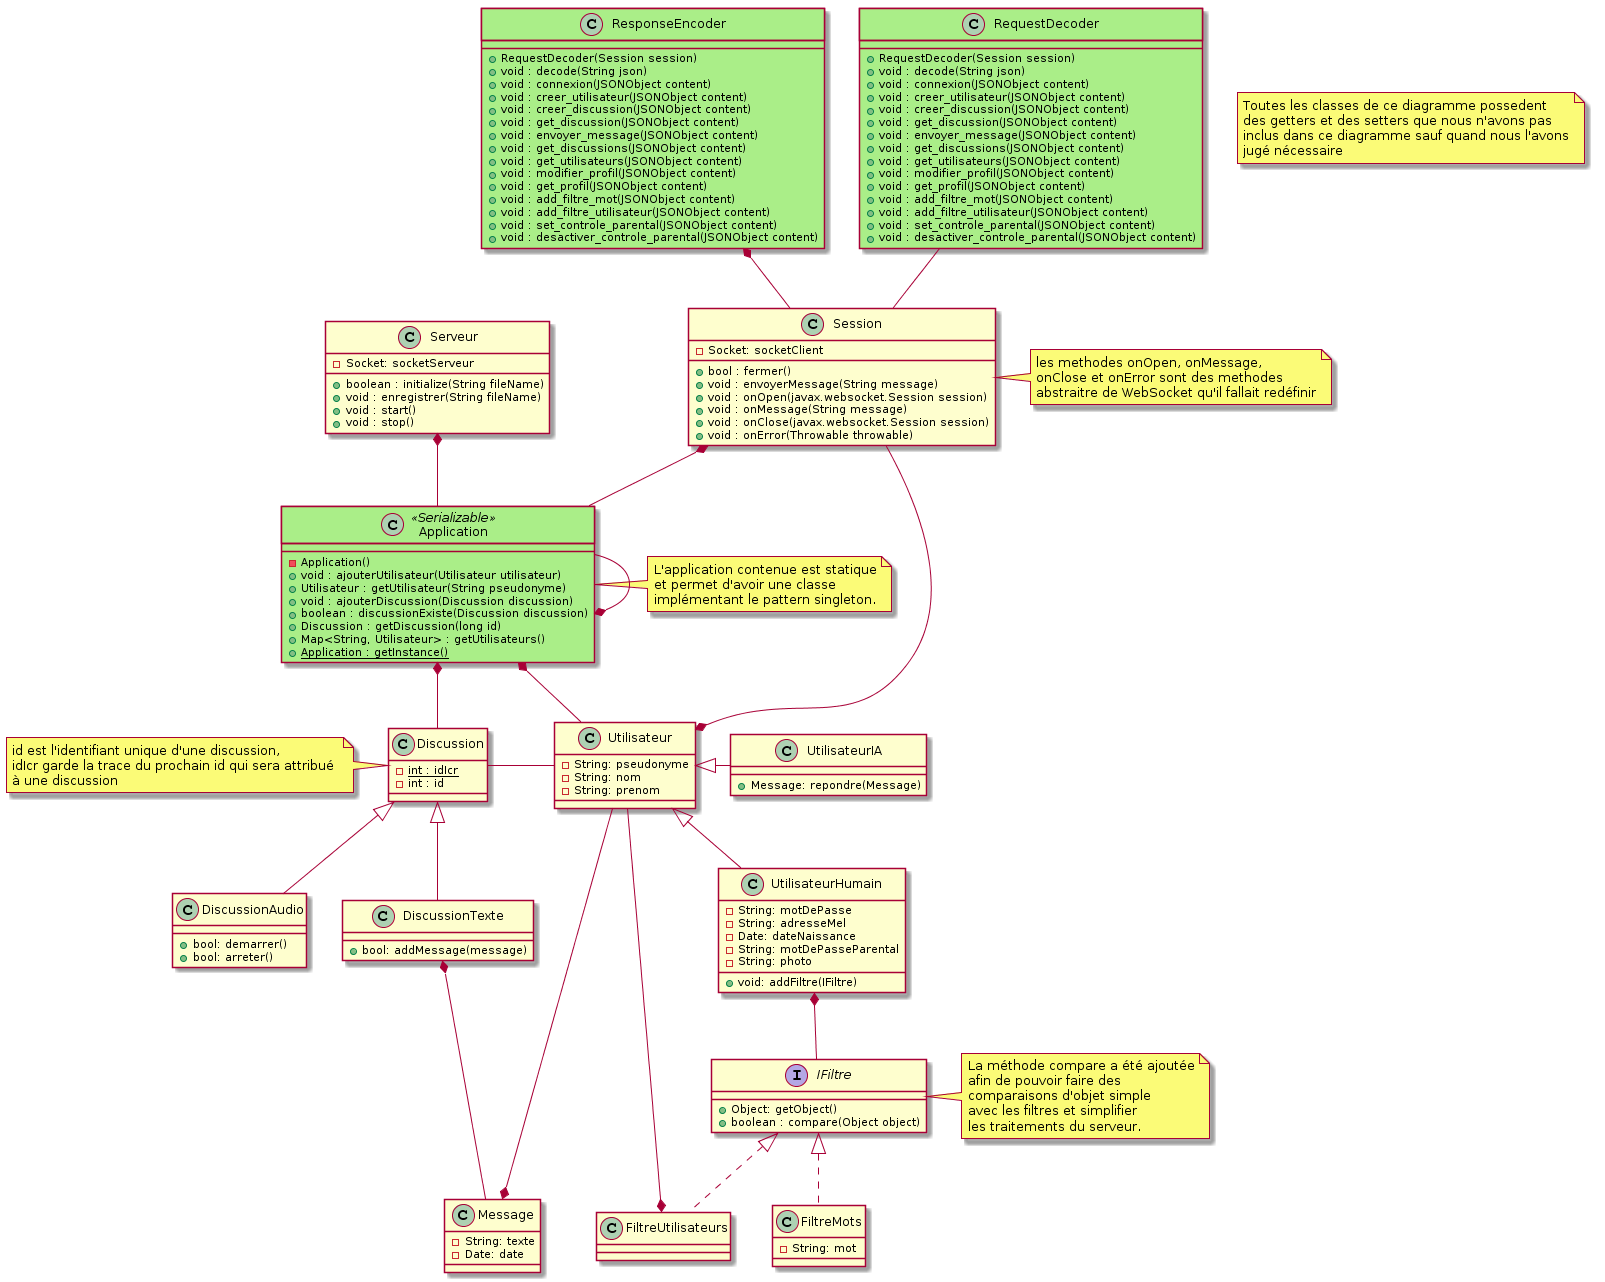
\includegraphics[width=19cm]{img/classesServeurV2.png}}
		\caption{Diagramme de classes côté serveur}
	\end{figure}

	\newpage

	Ce diagramme de classes représente la partie client de notre application, avec les attributs et méthodes des différentes classes.
	Les getter et setter ne sont pas présents sur celui-ci mais sont présents dans l'implémentation.
	
	%TODO diag à jour ??
	\begin{figure}[H]
		\centerline{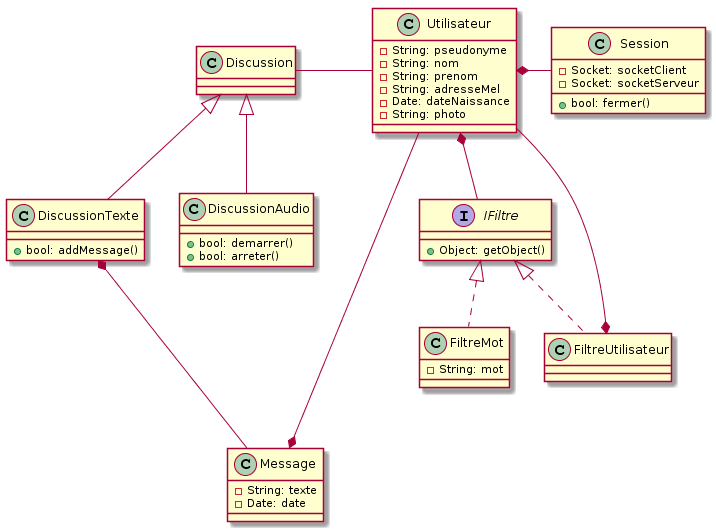
\includegraphics[width=16.5cm]{img/classesClient.png}}
		\caption{Diagramme de classes côté client}
	\end{figure}

